\documentclass{article}
\usepackage{amsmath}
\usepackage{amssymb}
\usepackage[dvipsnames]{xcolor}
\usepackage[margin=1.2in]{geometry}
\usepackage{graphicx}
\usepackage{tikz}
\usepackage{pgfplots}
\pgfplotsset{compat=1.11}

\newcommand*\Eval[3]{\left[#1\right]_{#2}^{#3}}

\begin{document}

\title{Theory of Probability HW \#2}
\author{Ozaner Hansha}
\date{September 23, 2019}
\maketitle

\begin{center}
    \Large{\textbf{Part A}}
\end{center}
Problems taken from Chapters 2 and 3 of the textbook.

\section*{\underline{Chapter 2}}

\section*{Problem 31a}
\noindent\textbf{Problem:} A 3-person basketball team consists of a guard, a forward, and a center. If a person is chosen at random from each of three different such teams, what is the probability of selecting a complete team? \textit{(use the inclusion-exclusion principle instead of calculating directly)}
\bigskip

\noindent\textbf{Solution:} Let $G$ denote the chosen team has 1 guard, $F$ denote that it was onw forward, and $C$ denote that it has one center. Then the probability we seek is $P(GFC)$. Note that we can express this in terms of the probability of the union of events:

\begin{align*}
    P(GFC)&=P(((GFC)^\complement)^\complement)\tag{involutory property}\\
    &=P((G^\complement\cup F^\complement\cup C^\complement)^\complement)\tag{DeMorgan's law}\\
    &=1-P(G^\complement\cup F^\complement\cup C^\complement)\tag{complement of event}
\end{align*}

Via the inclusion-exclusion principle for $n=3$ we have:

\begin{align*}
    P(G^\complement\cup F^\complement\cup C^\complement)&=P(G^\complement)+P(F^\complement)+P(C^\complement)\\
    &-P(G^\complement F^\complement)-P(G^\complement C^\complement)-P(F^\complement C^\complement)\\
    &+P(G^\complement F^\complement C^\complement)
\end{align*}

Now note that the probability that any particular position is not chosen from any particular team is $\frac{2}{3}$ since there are 2 valid options out of the 3 members. Since there are 3 teams the principle of counting gives us:

\begin{equation*}
    P(G^\complement)=P(F^\complement)=P(C^\complement)=\frac{2}{3}\cdot\frac{2}{3}\cdot\frac{2}{3}=\frac{2^3}{3^3}
\end{equation*}

In a similar vain, the probability that any 2 different positions are not chosen from any particular team is $\frac{1}{3}$ since there is only 1 valid option out of the 3 members. Since there are 3 teams the principle of counting gives us:

\begin{equation*}
    P(G^\complement F^\complement)=P(G^\complement C^\complement)=P(F^\complement C^\complement)=\frac{1}{3}\cdot\frac{1}{3}\cdot\frac{1}{3}=\frac{1}{3^3}
\end{equation*}

And taken to the extreme, the probability that none of the three positions are chosen from any particular team is 0 since each member has a position and at least 1 member from each team must be chosen:

\begin{equation*}
    P(G^\complement F^\complement C^\complement)=0\cdot0\cdot0=0
\end{equation*}

Plugging this into the inclusion-exclusion principle we have:

\begin{align*}
    P(G^\complement\cup F^\complement\cup C^\complement)&=\frac{2^3}{3^3}+\frac{2^3}{3^3}+\frac{2^3}{3^3}-\frac{1}{3^3}-\frac{1}{3^3}-\frac{1}{3^3}+0\\
    &=\frac{3\cdot2^3}{3^3}-\frac{3}{3^3}=\frac{7}{9}
\end{align*}

And so our desired probability is given by:

\begin{equation*}
    P(GFC)=1-P(G^\complement\cup F^\complement\cup C^\complement)=1-\frac{7}{9}=\frac{2}{9}
\end{equation*}

\section*{Problem 45}
\noindent\textbf{Problem:} A woman has $n$ keys, of which only 1 will open her door. \textbf{a)} If she tries keys at random, discarding those that do not work, what's the probability she will open the door on her $k$th try? \textbf{b)} What if she doesn't discard the keys?
\bigskip

\noindent\textbf{Solution:} Let $E_k$ be the event she opens the door on the $k$th key. \textbf{a)} Note that the first try has a $\frac{1}{n}$ chance of being correct, the second has a $P(E_1^\complement)\frac{1}{n-1}$ chance since the first try had to fail and since 1 key has been discarded, and so on. This pattern gives us:

\begin{align*}
    P(E_1)&=\frac{1}{n}\\
    P(E_2)&=\underbrace{\frac{n-1}{n}}_{P(E_1^\complement)}\cdot\frac{1}{n-1}\\
    P(E_3)&=\underbrace{\frac{n-1}{n}}_{P(E_1^\complement)}\cdot\underbrace{\frac{n-2}{n-1}}_{P(E_2^\complement)}\cdot\frac{1}{n-2}\\
    &\setbox0\hbox{=}\mathrel{\makebox[\wd0]{\hfil\vdots\hfil}}\\
    P(E_k)&=\underbrace{\frac{n-1}{n}}_{P(E_1^\complement)}\cdot\underbrace{\frac{n-2}{n-1}}_{P(E_2^\complement)}\cdots\underbrace{\frac{n-k+1}{n-k+2}}_{P(E_{k-1}^\complement)}\cdot\frac{1}{n-k+1}
\end{align*}

It is quite plain to see that this is a finite telescoping product. Canceling out the like factors, we are left with the very simple:

\begin{equation*}
    P(E_k)=\frac{1}{n}
\end{equation*}

\textbf{b)} If she doesn't discard the keys, then each try is independent of any other. And so the probability of her opening the door on the $k$th try is the probability that she failed the first $k-1$ tries then succeeded $k$th one:

\begin{equation*}
    P(E_k)=\left(\frac{n-1}{n}\right)^{k-1}\frac{1}{n}
\end{equation*}

\section*{Problem 55a}
\noindent\textbf{Problem:} What's the probability that a hand of 13 cards contains both ace and king of at least one suit?
\bigskip

\noindent\textbf{Solution:} Let $E_\heartsuit$ denote the event that our hand has both an ace and king of hearts, $E_\spadesuit$ denote the event that our hand has both an ace and king of diamonds, and so on. Thus, we desire the probability of the following event $E_\heartsuit\cup E_\spadesuit\cup E_\diamondsuit\cup E_\clubsuit$. The cardinality of this event is given by the inclusion-exclusion principle:

\begin{equation*}
    |E_\heartsuit\cup E_\spadesuit\cup E_\diamondsuit\cup E_\clubsuit|=\left|\bigcup_{i\in\{\heartsuit,\spadesuit,\diamondsuit,\clubsuit\}}\mkern-30muE_i\mkern+10mu\right|=\sum_{k=1}^4\left((-1)^{k-1}\mkern-10mu\sum _{I\subseteq \{\heartsuit,\spadesuit,\diamondsuit,\clubsuit\} \atop |I|=k}\left|\bigcap_{i\in I}E_i\right|\right)
\end{equation*}

Now note that each suit we have determines 2 of the cards in our hand. For example, $|E_\heartsuit|=\binom{52-2}{13-2}$ since 2 of the cards have been chosen for us. Similarly, we have $|E_\heartsuit E_\spadesuit|=\binom{52-4}{13-4}$ since 4 of the cards (2 from hearts and 2 from spades) have been chosen for us. Generalizing this, we have for $|I|=k$:

\begin{equation*}
    \left|\bigcap_{i\in I}E_i\right|=\binom{52-2k}{13-2k}
\end{equation*}

Plugging this into our expression for the inclusion-exclusion principle gives us:

\begin{equation*}
    \left|\bigcup_{i\in\{\heartsuit,\spadesuit,\diamondsuit,\clubsuit\}}\mkern-30muE_i\mkern+10mu\right|=\sum_{k=1}^4\left((-1)^{k-1}\mkern-10mu\sum _{I\subseteq \{\heartsuit,\spadesuit,\diamondsuit,\clubsuit\} \atop |I|=k}\binom{52-2k}{13-2k}\right)
\end{equation*}

Now, noting that there are $\binom{4}{k}$ $k$-combinations of the set $\{\heartsuit,\spadesuit,\diamondsuit,\clubsuit\}$, we have:

\begin{equation*}
    \left|\bigcup_{i\in\{\heartsuit,\spadesuit,\diamondsuit,\clubsuit\}}\mkern-30muE_i\mkern+10mu\right|=\sum_{k=1}^4\left((-1)^{k-1}\binom{4}{k}\binom{52-2k}{13-2k}\right)=139565328072
\end{equation*}

We have calculated the number of hands with at least 1 pair of an ace and heart of a single suit. And because this is a discrete uniform distribution, i.e. each hand is equally likely, the probability of drawing such a hand is simply:

\begin{equation*}
    P(E_\heartsuit\cup E_\spadesuit\cup E_\diamondsuit\cup E_\clubsuit)=\frac{|E_\heartsuit\cup E_\spadesuit\cup E_\diamondsuit\cup E_\clubsuit|}{|\Omega|}=\frac{139565328072}{\binom{52}{13}}=\frac{9895443}{45023650}\approx0.219783
\end{equation*}

\section*{\underline{Chapter 3}}

\section*{Problem 12}
\noindent\textbf{Problem:} Suppose distinct values are written on each of 3 cards, which are then randomly named $a,b$, and $c$. Given that $a< b$ find the probability that $a<c$. 
\bigskip

\noindent\textbf{Solution:} Note that we can consider the sample space $\Omega$ of this experiment the $3!$ passive permutations of $\{a,b,c\}$:

\begin{equation*}
    \Omega=\{(a,b,c),(a,c,b),(b,a,c),\cdots\}
\end{equation*}

The event $E_{a<b}$ is given by the set of all triplets in $\Omega$ in which $a$ precedes $b$:

\begin{equation*}
    E_{a< b}=\{(a,b,c),(a,c,b),(c,a,b)\}
\end{equation*}

The event $E_{a< c}$ is given by the set of all triplets in $\Omega$ in which $a$ precedes $c$:

\begin{equation*}
    E_{a< c}=\{(a,b,c),(a,c,b),(b,a,c)\}
\end{equation*}

The intersection of these two events $E_{a<b}E_{a<c}$ is thus given by:

\begin{equation*}
    E_{a<b}E_{a< c}=\{(a,b,c),(a,c,b)\}
\end{equation*}

And now, noting that this is a discrete uniform distribution, we can finally calculate the desired conditional probability of $a<c$ assuming $a<b$:

% \begin{equation*}
%     P(E_{a<c}| E_{a<b})=\frac{P(E_{a<b}E_{a< c})}{P(E_{a<b})}=\frac{{|E_{a<b}E_{a< c}|}/{|\Omega|}}{{|E_{a<b}|}/{|\Omega|}}=\frac{{2}/{3!}}{{3}/{3!}}=\frac{2}{3}
% \end{equation*}

\begin{equation*}
    P(E_{a<c}| E_{a<b})=\frac{|E_{a<b}E_{a< c}|}{|E_{a<b}|}=\frac{2}{3}
\end{equation*}

\section*{Problem 30}
\noindent\textbf{Problem:} Suppose that a deck of 52 cards is shuffled and the cards are then turned over one at a time until the first ace appears. Given that the first ace is the 20th card, what is the conditional probability that the card following it is \textbf{a)} the ace of spades? \textbf{b)} the two of clubs?
\bigskip

\noindent\textbf{Solution:} Let $A$ denote the event that the first ace drawn is the 20th card, $B$ denote that the 21st card is the ace of spades, and $C$ denote that the 21st card is the two of clubs. The cardinality of $A$ is given by:

\begin{equation*}
    |A|=\overbrace{\underbrace{48}_{\text{c1}}\cdot
    \underbrace{47}_{\text{c2}}\cdot
    \underbrace{46}_{\text{c3}}\cdots
    \underbrace{30}_{\text{c19}}}^{\substack{\text{non-ace}\\\text{cards}}}\cdot\overbrace{\underbrace{4}_{\text{c20}}}^{\substack{\text{ace}\\\text{cards}}}\cdot\overbrace{\underbrace{32!}_{\text{c21-c52}}}^{\substack{\text{all other}\\\text{cards}}}=48^{\underline{19}}\cdot 4\cdot 32!
\end{equation*}

Via similar reasoning, the cardinality of $BA$ is given by:

\begin{equation*}
    |BA|=\overbrace{\underbrace{48}_{\text{c1}}\cdot
    \underbrace{47}_{\text{c2}}\cdot
    \underbrace{46}_{\text{c3}}\cdots
    \underbrace{30}_{\text{c19}}}^{\substack{\text{non-ace}\\\text{cards}}}\cdot
    \overbrace{\underbrace{3}_{\text{c21}}}^{\substack{\text{aces of}\\\diamondsuit,\clubsuit,\heartsuit}}\cdot
    \overbrace{\underbrace{1}_{\text{c21}}}^{\text{ace of }\spadesuit}\cdot
    \overbrace{\underbrace{31!}_{\text{c22-c52}}}^{\substack{\text{all other}\\\text{cards}}}
    =48^{\underline{19}}\cdot 3\cdot 1\cdot 31!
\end{equation*}

Yet again via similar reasoning, the cardinality of $CA$ is given by:

\begin{equation*}
    |CA|=\overbrace{\underbrace{47}_{\text{c1}}\cdot
    \underbrace{46}_{\text{c2}}\cdot
    \underbrace{45}_{\text{c3}}\cdots
    \underbrace{29}_{\text{c19}}}^{\substack{\text{non-ace/two of }{\clubsuit}\\\text{cards}}}\cdot
    \overbrace{\underbrace{4}_{\text{c20}}}^{\substack{\text{ace}\\\text{cards}}}\cdot
    \overbrace{\underbrace{1}_{\text{c21}}}^{\text{two of }\clubsuit}\cdot
    \overbrace{\underbrace{31!}_{\text{c22-c52}}}^{\substack{\text{all other}\\\text{cards}}}
    =47^{\underline{19}}\cdot 4\cdot 31!
\end{equation*}

The probabilities we seek are \textbf{a)} $P(B| A)$ and \textbf{b)} $P(C| A)$ and since this is a discrete uniform distribution, we have:

\begin{align*}
    P(B| A)&=\frac{|BA|}{|A|}=\frac{48^{\underline{19}}\cdot 3\cdot 1\cdot 31!}{48^{\underline{19}}\cdot 4\cdot 32!}=\frac{3}{4\cdot 32}=\frac{3}{128}\\
    P(C| A)&=\frac{|CA|}{|A|}=\frac{47^{\underline{19}}\cdot 4\cdot 31!}{48^{\underline{19}}\cdot 4\cdot 32!}=\frac{29}{48\cdot 32}=\frac{29}{1536}
\end{align*}

\section*{Problem 35}
\noindent\textbf{Problem:} On rainy days Joe is late to work with probability 0.3, and on nonrainy days he is late with probability 0.1. It will rain tomorrow with probability 0.7. \textbf{a)} Find the probability that Joe is early tomorrow. \textbf{b)} Given that Joe is early, what is the conditional probability that it rained?
\bigskip

\noindent\textbf{Solution:} Let $L$ denote the event that joe is late, and $R$ denote the event that it is raining. The problem statement and the complement rule gives us the following probabilities:

\begin{align*}
    P(R)&=0.7\,\,\,\,\,\,\,P(R^\complement)=0.3\\
    P(L| R)&=0.3\,\,\,\,\,\,\,P(L| R^\complement)=0.1
\end{align*}

Now note that via the law of total probability, $P(L)$ is given by:

\begin{align*}
    P(L)&=P(L| R)P(R)+P(L| R^\complement)P(R^\complement)\\
    &=0.3\cdot0.7+0.1\cdot0.3=0.24
\end{align*}

And so for \textbf{a)} the probability that Joe is early (i.e. not late) is given by:

\begin{equation*}
    P(L^\complement)=1-P(L)=1-0.24=0.76
\end{equation*}

For \textbf{b)} the desired probability is given by $P(R| L^\complement)$. We can solve for this probability via Bayes' theorem:

\begin{align*}
    P(R| L^\complement)&=\frac{P(L^\complement| R)P(R)}{P(L^\complement)}\tag{Bayes' theorem}\\
    &=\frac{(1-P(L| R))P(R)}{P(L^\complement)}\tag{complement of conditional}\\
    &=\frac{(1-0.3)0.7}{0.76}=\frac{49}{76}\approx0.644734
\end{align*}

\section*{Problem 47a}
\noindent\textbf{Problem:} There is a 30\% chance that $A$ can fix her busted computer. If $A$ cannot, then there is a 40\% chance that her friend $B$ can fix it. Find the probability it will be fixed by either $A$ or $B$.
\bigskip

\noindent\textbf{Solution:} Let $A$ denote the probability that she fixes the computer, and $B$ denote that the friend fixes the computer. Thus the problem statement gives us:

\begin{equation*}
    P(A)=0.3\,\,\,\,\,\,\,\,P(B| A^\complement)=0.4
\end{equation*}
\pagebreak

Now, note that by Bayes' theorem we have the following chain of equalities:

\begin{align*}
    P(B|A^\complement)&=\frac{P(A^\complement| B)P(B)}{P(A^\complement)}\tag{Bayes' theorem}\\
    0.4&=\frac{P(A^\complement| B)P(B)}{1-0.3}\\
    0.4\cdot0.7&=P(A^\complement| B)P(B)\\
    0.28&=(1-P(A| B))P(B)\tag{complement of conditional}\\
    0.28&=P(B)-P(A| B)P(B)\\
    0.28&=P(B)-P(AB)\tag{def. of conditional probability}
\end{align*}

Now, via the inclusion-exclusion principle for $n=2$, we can solve for our desired probability, that either $A$ or $B$ fix the computer, $P(A\cup B)$ :

\begin{equation*}
    P(A\cup B)=P(A)+P(B)-P(AB)=0.3+0.28=0.58
\end{equation*}
\bigskip

\begin{center}
    \Large\textbf{Part B}
\end{center}

\begin{center}
    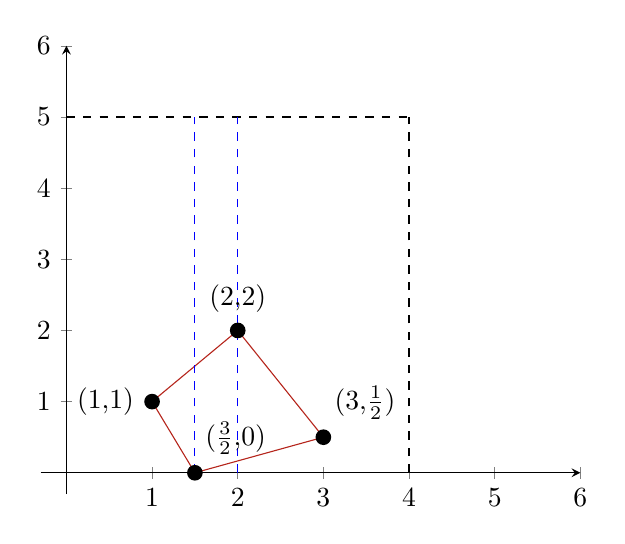
\begin{tikzpicture}
    \begin{axis}[
        xmin=-.3,xmax=6,
        ytick = {0,1,...,6},
        ymin=-.3,ymax=6,
        axis lines=center,
        legend style={legend cell align=right,legend plot pos=right}] 
    \addplot[color=BrickRed,domain=3/2:3,samples=100] {x/3-1/2};
    \addplot[color=BrickRed,domain=1:2,samples=100] {x};
    \addplot[color=BrickRed,domain=2:3,samples=100] {-3*x/2+5};
    \addplot[color=BrickRed,domain=1:3/2,samples=100] {-2*x+3};
    \draw [dashed] (4,0) -- (4,5);
    \draw [dashed] (0,5) -- (4,5);
    \draw [dashed,color=blue] (3/2,0) -- (3/2,5);
    \draw [dashed,color=blue] (2,0) -- (2,5);
    \node[label={180:{(1,1)}},circle,fill,inner sep=2pt] at (axis cs:1,1) {};
    \node[label={90:{(2,2)}},circle,fill,inner sep=2pt] at (axis cs:2,2) {};
    \node[label={86:{($\frac{3}{2}$,0)}},circle,fill,inner sep=2pt] at (axis cs:3/2,0) {};
    \node[label={80:{(3,$\frac{1}{2}$)}},circle,fill,inner sep=2pt] at (axis cs:3,1/2) {};
    \end{axis}
    \end{tikzpicture}
\end{center}

\section*{Problem a}
\noindent\textbf{Problem:} Express the area in the red bounded region $E$ as a sum of integrals.
\bigskip

\noindent\textbf{Solution:} As we can see, the red bounded region can be expressed as the 3 regions split up by the blue dashed lines. The functions of each side, starting with the top left line and going clockwise, are given by: 
\begin{align*}
    y&=x\\
    y&=\frac{-3x}{2}+5\\
    y&=\frac{x}{3}-\frac{1}{2}\\
    y&=-2x+3
\end{align*}
\pagebreak

And so we can express our integral sum like so:

\begin{equation*}
    \int_{1}^{\frac{3}{2}}\int_{-2x+3}^{x}\mathop{dy}\mathop{dx}+
    \int^{2}_{\frac{3}{2}}\int_{\frac{x}{3}-\frac{1}{2}}^{x}\mathop{dy}\mathop{dx}+
    \int_{2}^{3}\int_{\frac{x}{3}-\frac{1}{2}}^{\frac{-3x}{2}+5}\mathop{dy}\mathop{dx}
\end{equation*}

\section*{Problem b}
\noindent\textbf{Problem:} Compute the area of $E$.
\bigskip

\noindent\textbf{Solution:} Computing the integral sum, we have:

\begin{align*}
    &\phantom{=}\int_{1}^{\frac{3}{2}}\int_{-2x+3}^{x}\mathop{dy}\mathop{dx}+
    \int^{2}_{\frac{3}{2}}\int_{\frac{x}{3}-\frac{1}{2}}^{x}\mathop{dy}\mathop{dx}+
    \int_{2}^{3}\int_{\frac{x}{3}-\frac{1}{2}}^{\frac{-3x}{2}+5}\mathop{dy}\mathop{dx}\\
    &=\int_{1}^{\frac{3}{2}}\Eval{y}{-2x+3}{x}\mathop{dx}+
    \int^{2}_{\frac{3}{2}}\Eval{y}{\frac{x}{3}-\frac{1}{2}}{x}\mathop{dx}+
    \int_{2}^{3}\Eval{y}{\frac{x}{3}-\frac{1}{2}}{\frac{-3x}{2}+5}\mathop{dx}\\
    &=\int_{1}^{\frac{3}{2}}3x-3\mathop{dx}+
    \int^{2}_{\frac{3}{2}}\frac{2x}{3}+\frac{1}{2}\mathop{dx}+
    \int_{2}^{3}\frac{-11x}{6}+\frac{11}{2}\mathop{dx}\\
    &=\Eval{\frac{3x^2}{2}-3x}{1}{\frac{3}{2}}+
    \Eval{\frac{2x^2}{6}+\frac{x}{2}}{2}{\frac{3}{2}}+
    \Eval{\frac{-11x^2}{12}+\frac{11x}{2}}{2}{3}\\
    &=\frac{3}{8}+\frac{5}{6}+\frac{11}{12}=\frac{17}{8}
\end{align*}

\section*{Problem c}
\noindent\textbf{Problem:} Suppose the rectangle $R$ (demarcated by the black dashed lines) represents the backyard of a house where a drone is trying to
drop a (very small) parcel, and $E$ represents a swimming pool in the backyard. If the drone drops the parcel in $R$ at random, what is the probability that the parcel will not fall in the swimming pool?
\bigskip

\noindent\textbf{Solution:} Assuming the parcel is point-like and that the area $R$ represents a uniform distribution, we can imagine that the probability the parcel lands in the pool $P(L)$ is given by:

\begin{equation*}
    P(L)=\frac{\text{Area of } E}{\text{Area of } R}=\frac{17}{8\cdot20}=\frac{17}{160}
\end{equation*}

And so the probability it doesn't fall in is simply the complement:

\begin{equation*}
    P(L^\complement)=1-P(L)=1-\frac{17}{160}=\frac{143}{160}
\end{equation*}

\end{document}